\label{sec:evaluation}

In this section, we conduct a comprehensive evaluation of POLAR-SGD under a realistic cross-datacenter (Cross-DC) training setting. 
% Our experiments are designed to answer the following questions:
% \begin{enumerate}
%     \item How much end-to-end training efficiency can POLAR-SGD deliver compared to a standard DP+PP baseline under WAN-like network constraints?
%     \item Does POLAR-SGD remain effective and robust in a multi-node, multi-GPU environment without relying on unrealistic hardware assumptions?
%     \item Does the throughput gain come at the expense of convergence behavior or final model quality?
%     \item Is a stabilization mechanism (e.g., error-correction) necessary beyond merely pipelining or relaxing synchronization?
% \end{enumerate}

\subsection{Experimental Setup}
\label{sec:setup}

Table~\ref{tab:setup} summarizes our experimental configuration. We compare POLAR-SGD against a standard implementation, denoted as \textbf{Baseline DDP (Standard DP+PP)}. This baseline employs a 1F1B pipeline schedule and performs a blocking All-Reduce to synchronize gradients at the end of each mini-batch. Under WAN-like Cross-DC conditions, such barriered synchronization typically induces substantial stalls and reduces effective GPU utilization.

In addition, we include a representative relaxed synchronization baseline, \textbf{LSGD ($k=4$)}, to highlight how delayed/local synchronization can alter training dynamics.

\subsection{Main Results}

We report end-to-end throughput in tokens/s in Table~\ref{tab:throughput}. For POLAR-SGD, we additionally report the normalized speedup over the Baseline DDP. 

\begin{table}[t]
    \caption{Experimental setup.}
    \label{tab:setup}
    \centering
    \begin{tabular}{@{}ll@{}}
        \toprule
        \textbf{Component} & \textbf{Specification} \\
        \midrule
        Model & LLaMA-2 7B \\
        Dataset & WikiText-103 \\
        Hardware & 32$\times$ NVIDIA A100 (40GB) GPUs \\
                 & across 4 nodes \\
        Network & Bandwidth: 30 Gb/s; RTT latency: 50 ms \\
        Parallelism & Hybrid DP+PP (PP=8, DP=4); \\
                    & batch=256; microbatch=32 \\
        Software & PyTorch 2.5; NCCL 2.23; CUDA 12.1 \\
        Metrics & Throughput (tokens/s), training loss \\
        \bottomrule
    \end{tabular}
\end{table}

\begin{table}[t]
    \caption{End-to-end throughput under Cross-DC network constraints.}
    \label{tab:throughput}
    \centering
    \begin{tabular}{@{}lcc@{}}
        \toprule
        \textbf{Method} & \textbf{Throughput (tokens/s)} & \textbf{Speedup} \\
        \midrule
        DDP+1F1B & 5,350 & 1.00$\times$ \\
        LSGD ($k=4$) & 9,433 & 1.76$\times$ \\
        POLAR-SGD & 10,016 & 1.87$\times$ \\
        \bottomrule
    \end{tabular}
\end{table}

\begin{figure}[t]
    \centering
    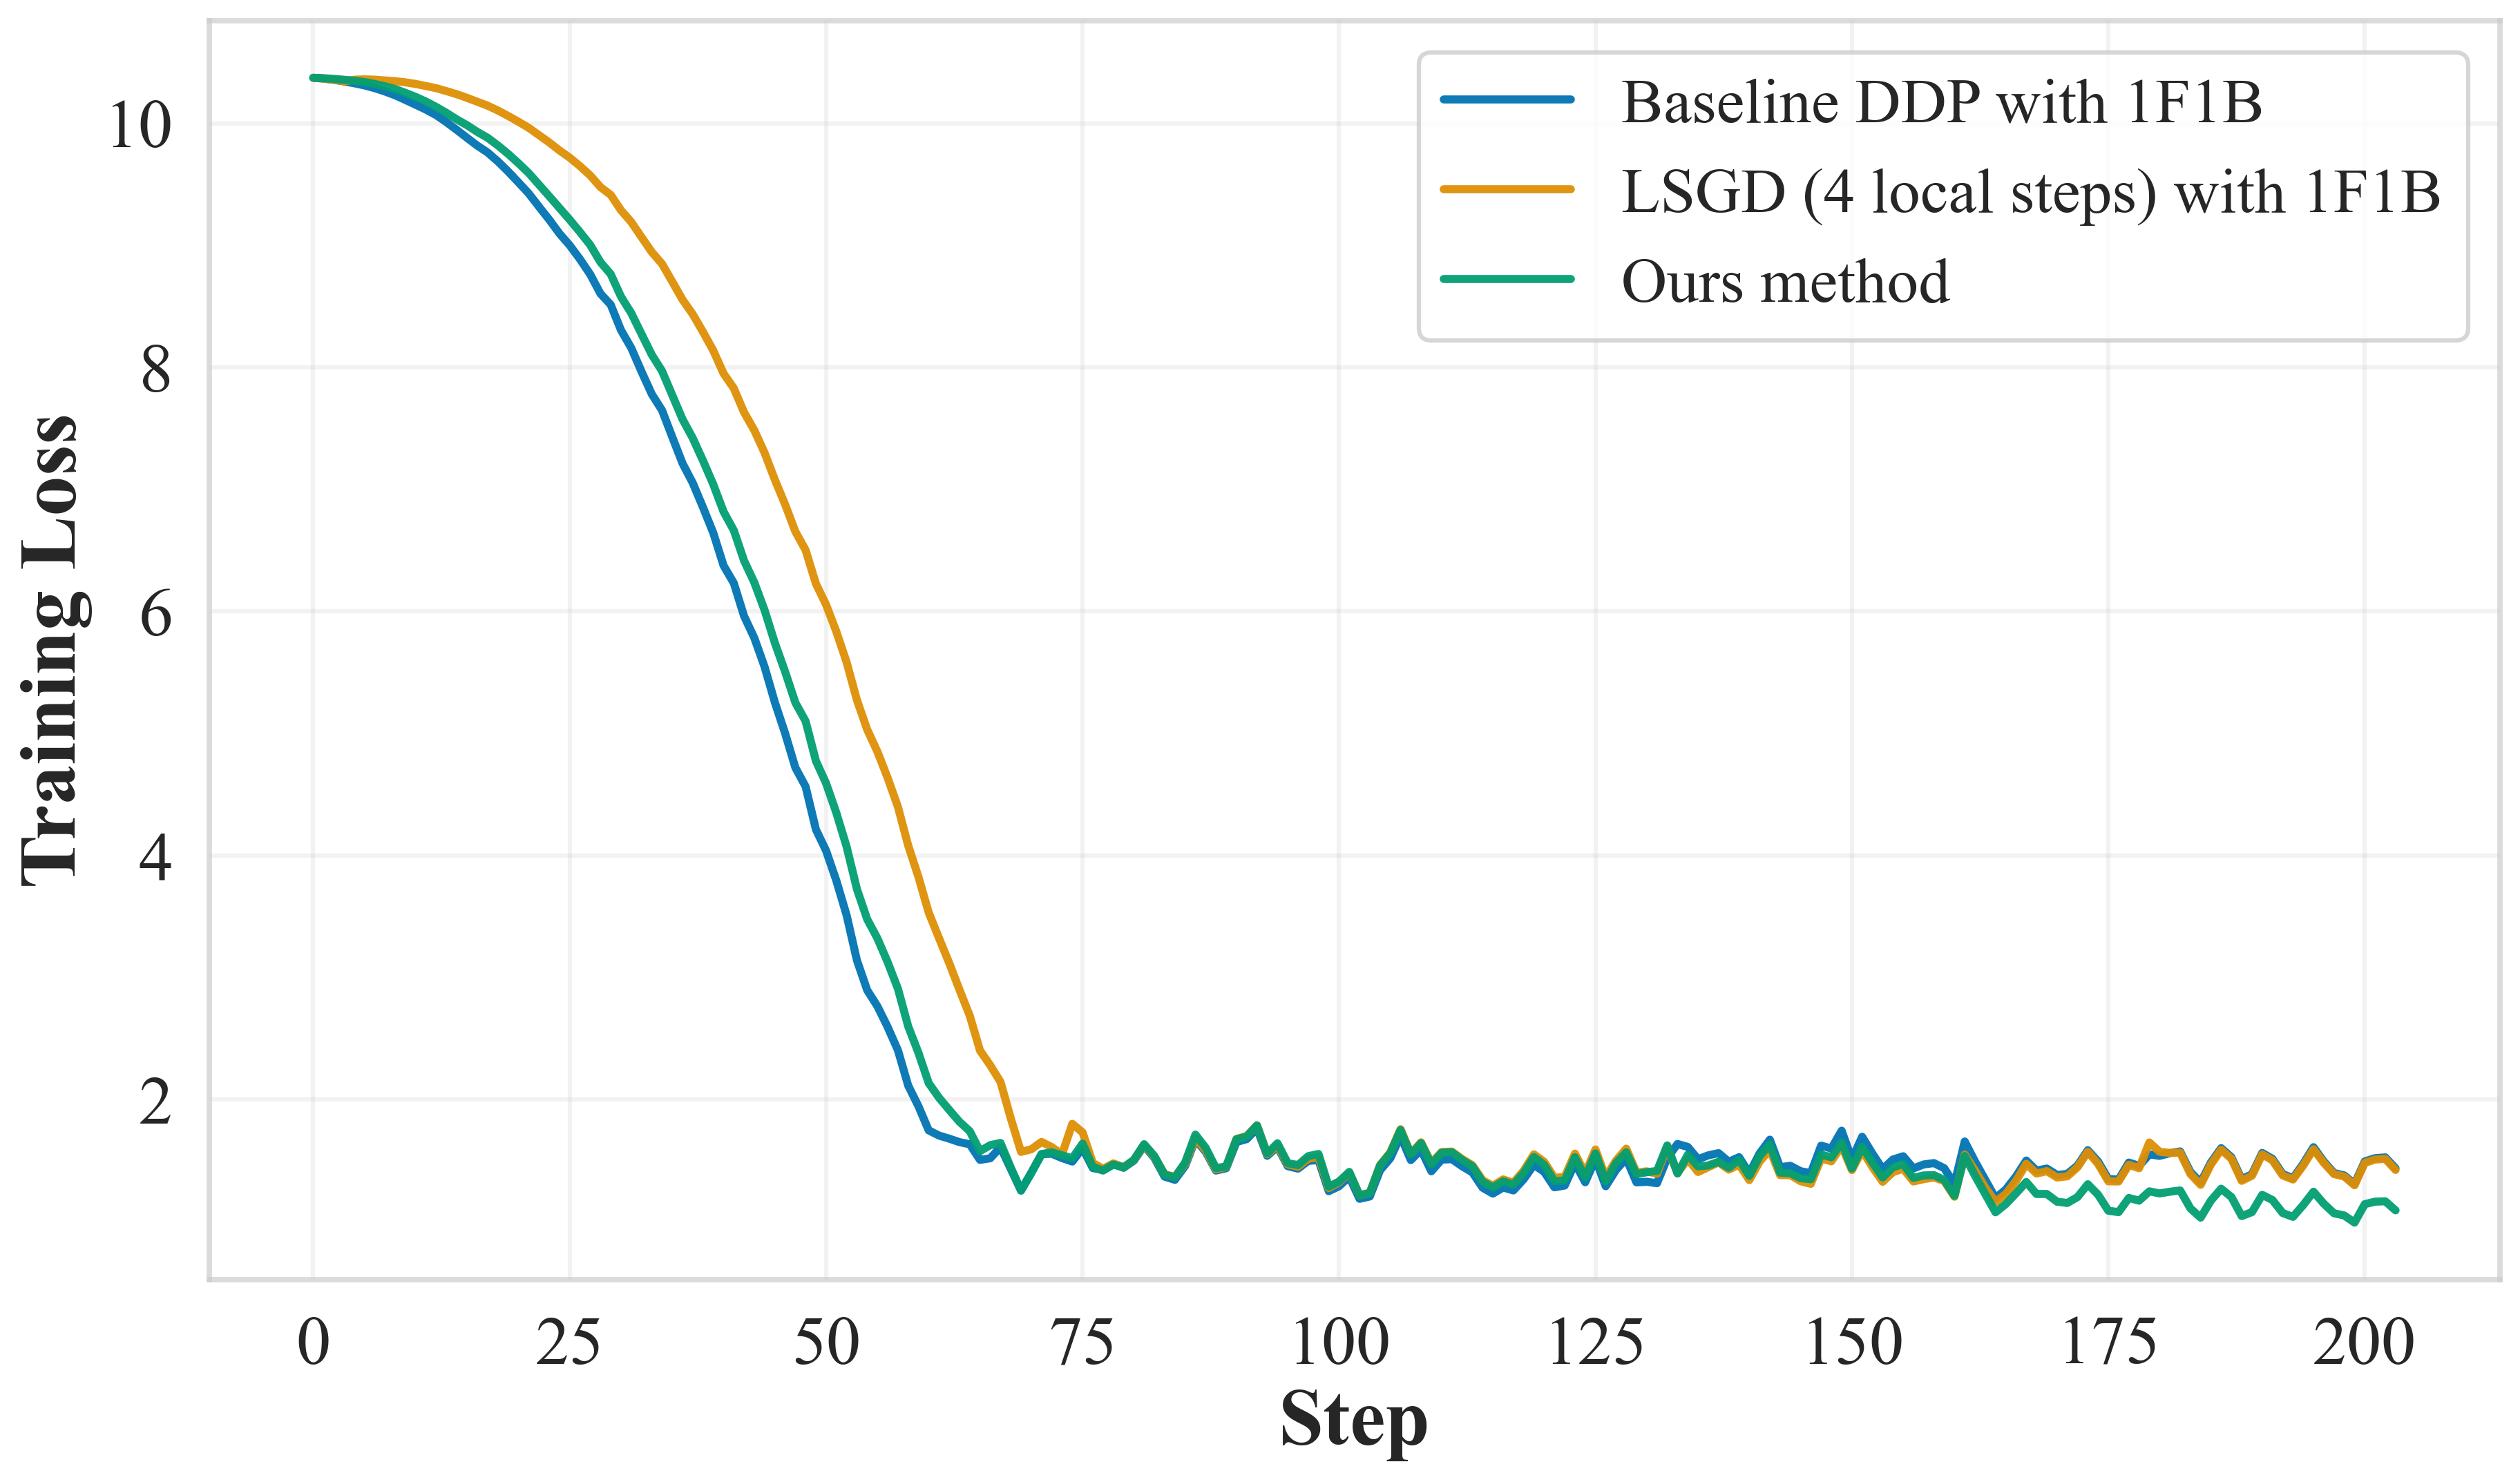
\includegraphics[width=\columnwidth]{images/json_curves_by_steps.png}
    \caption{Training loss versus steps on WikiText-103 (smoothed over a common step range). POLAR-SGD closely tracks the Baseline DDP, while LSGD shows a mild mid-to-late stage deviation, indicating that POLAR-SGD better preserves step-wise convergence stability under Cross-DC constraints.}
    \label{fig:loss_comparison}
\end{figure}

\begin{figure}[h]
    \centering
    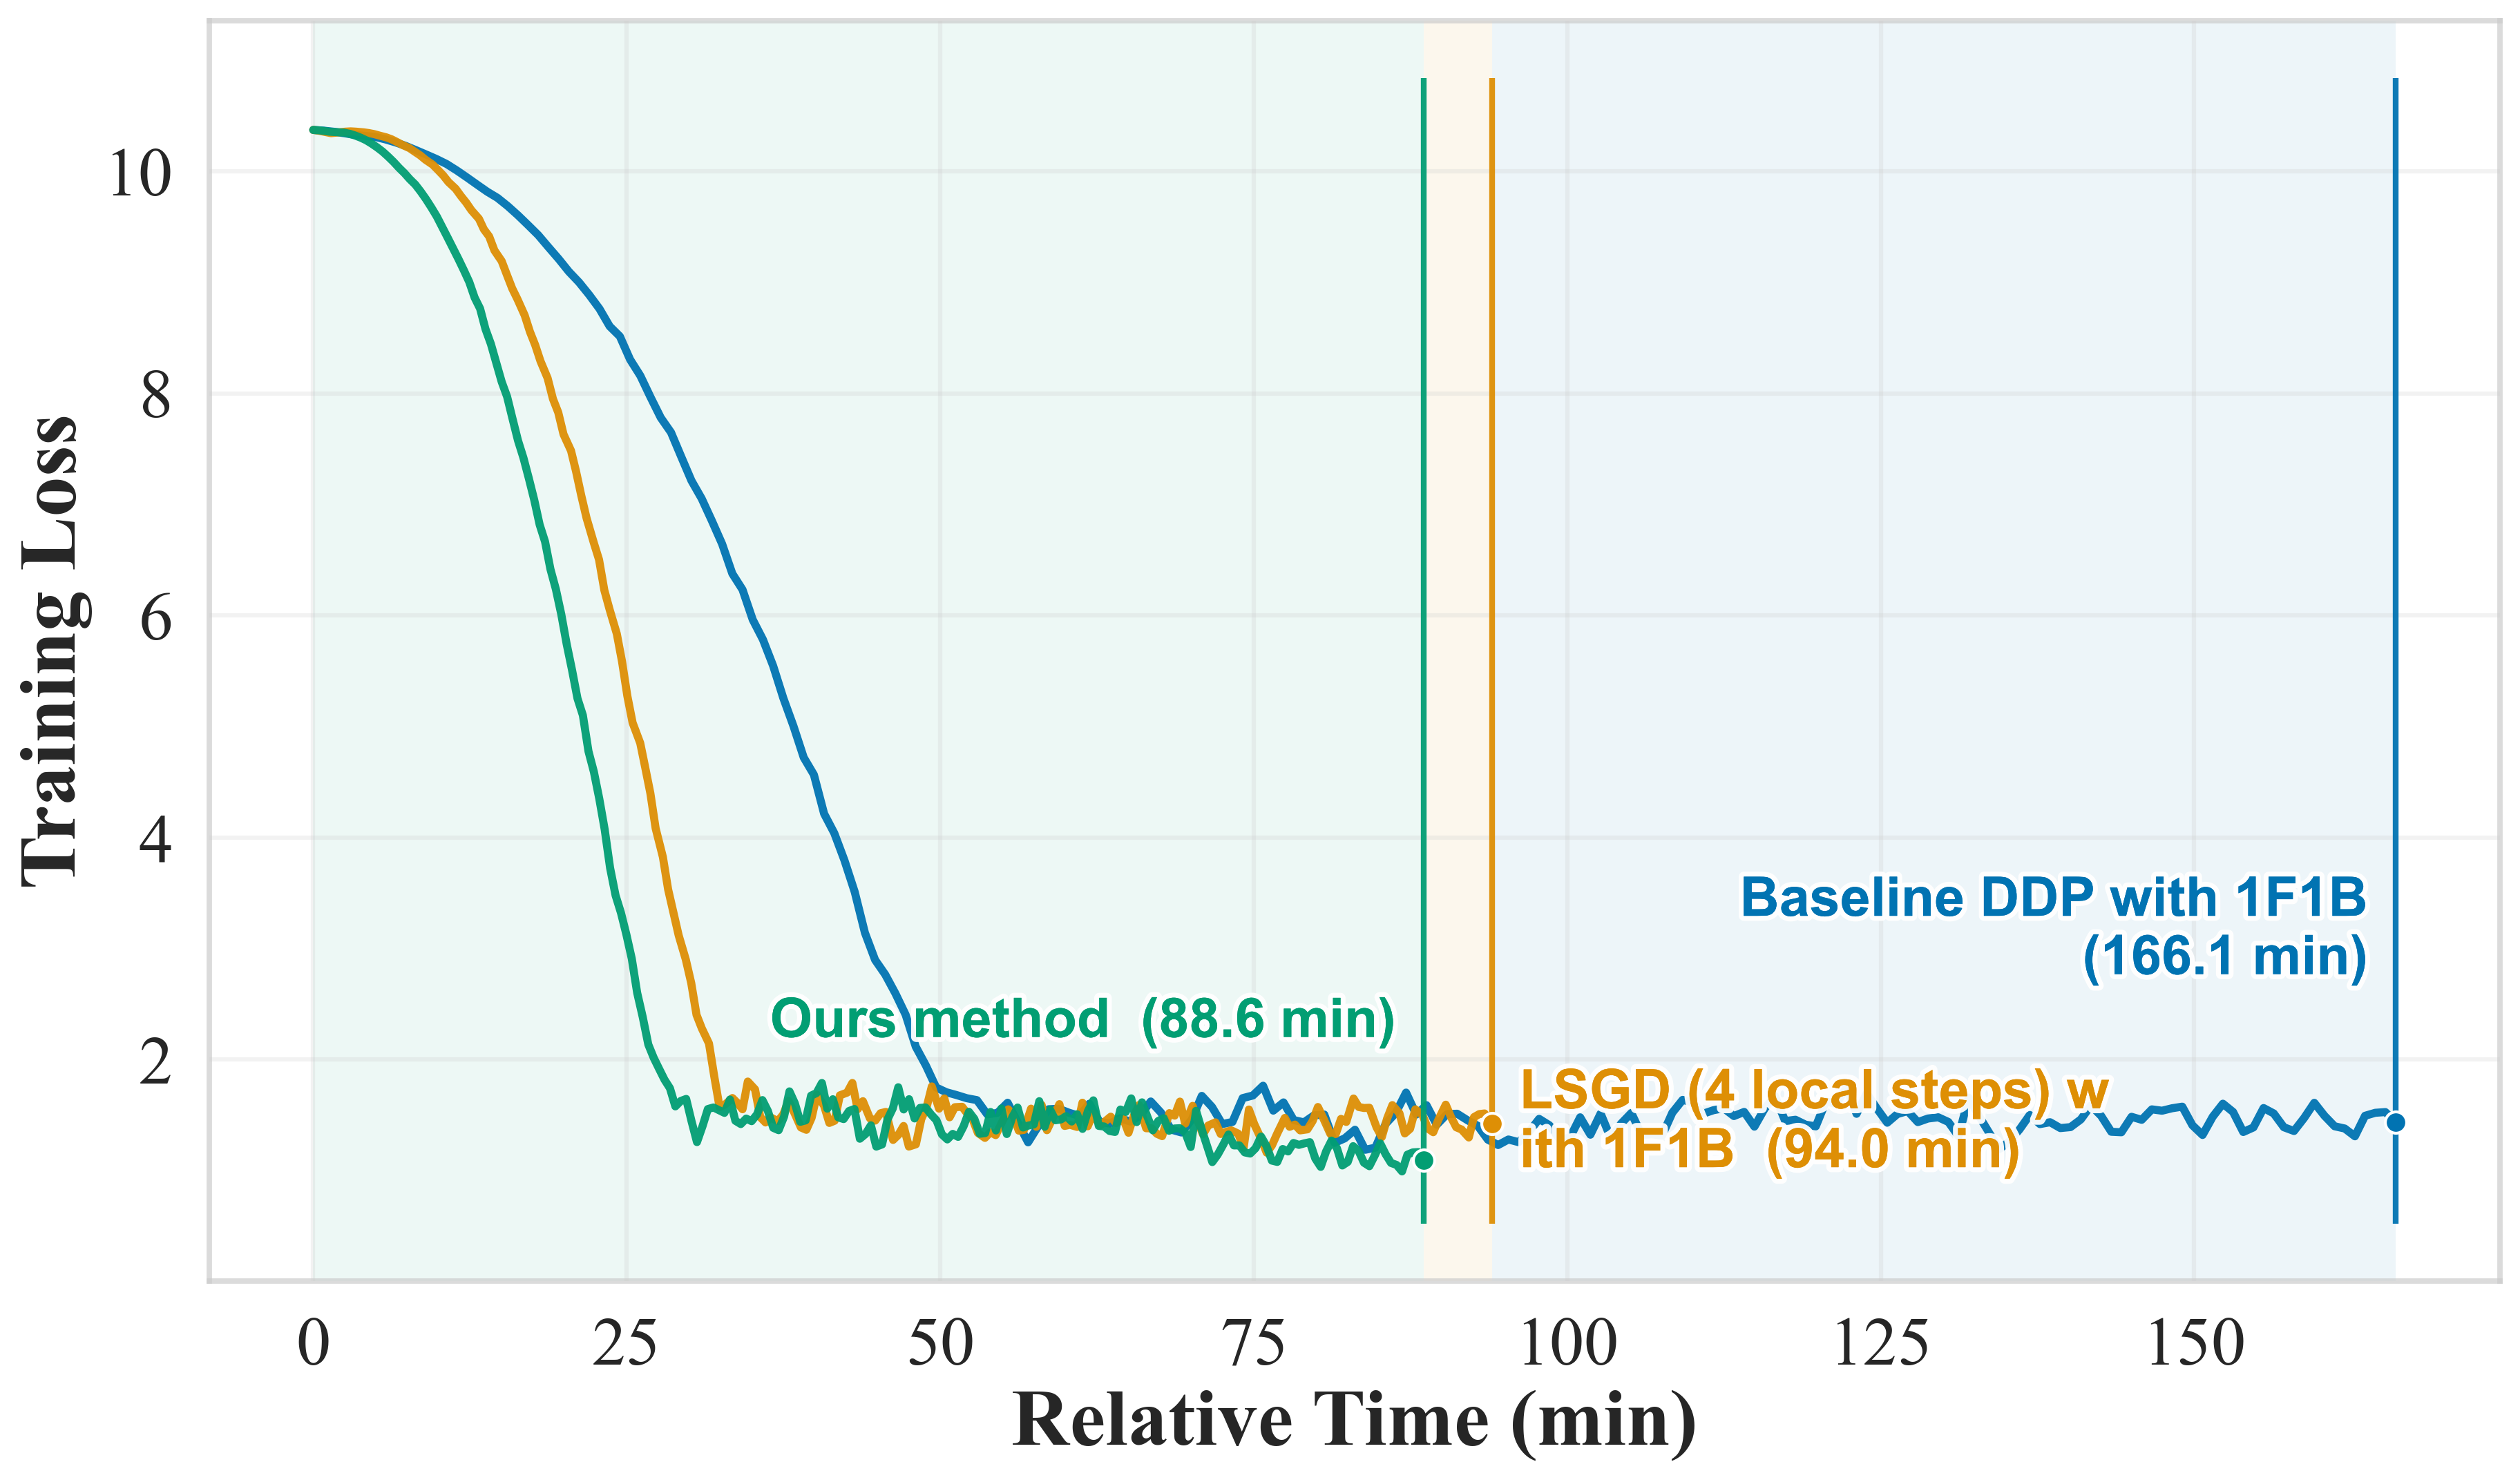
\includegraphics[width=\columnwidth]{images/json_curves_by_time.png}
    \caption{Training loss versus wall-clock time on WikiText-103 (smoothed). POLAR-SGD reaches the low-loss regime substantially earlier than the Baseline DDP, demonstrating improved time-to-target under Cross-DC network constraints.}
    \label{fig:loss_e2e_comparison}
\end{figure}

\paragraph{Convergence comparison by steps.}
Figure~\ref{fig:loss_comparison} reports the smoothed loss curves aligned by training steps over a common range. All methods exhibit a consistent overall trend: the loss decreases steadily and reaches a plateau after roughly 200 steps. Importantly, POLAR-SGD tracks the Baseline DDP closely across most of training, indicating that the proposed approach preserves stable optimization behavior despite introducing more aggressive communication/synchronization strategies. 

\paragraph{End-to-end convergence comparison by wall-clock time.}xs
The advantage of POLAR-SGD is more pronounced when comparing convergence as a function of wall-clock time. As shown in Figure~\ref{fig:loss_e2e_comparison}, POLAR-SGD reduces the loss substantially faster than the Baseline DDP under the same relative time budget. 
%Concretely, the baseline requires significantly longer time to reach a loss level comparable to POLAR-SGD, whereas POLAR-SGD enters the low-loss plateau much earlier. These results demonstrate that POLAR-SGD primarily improves \textbf{time-to-target}: even when step-wise convergence is similar, the reduced per-step overhead yields markedly better end-to-end training efficiency.

Taken together, Figures~\ref{fig:loss_comparison} and~\ref{fig:loss_e2e_comparison} support two conclusions. First, \textbf{convergence stability} is preserved: when aligned by steps, POLAR-SGD closely matches the baseline, showing no signs of instability or divergence. Second, \textbf{model quality is not sacrificed for throughput}: POLAR-SGD achieves comparable training loss while substantially reducing wall-clock time.


\subsection{Ablation Study}
\label{sec:ablation}

% NOTE: keep the ablation figure omitted until data is ready to avoid empty floats.
\begin{figure}[t]
    \centering
    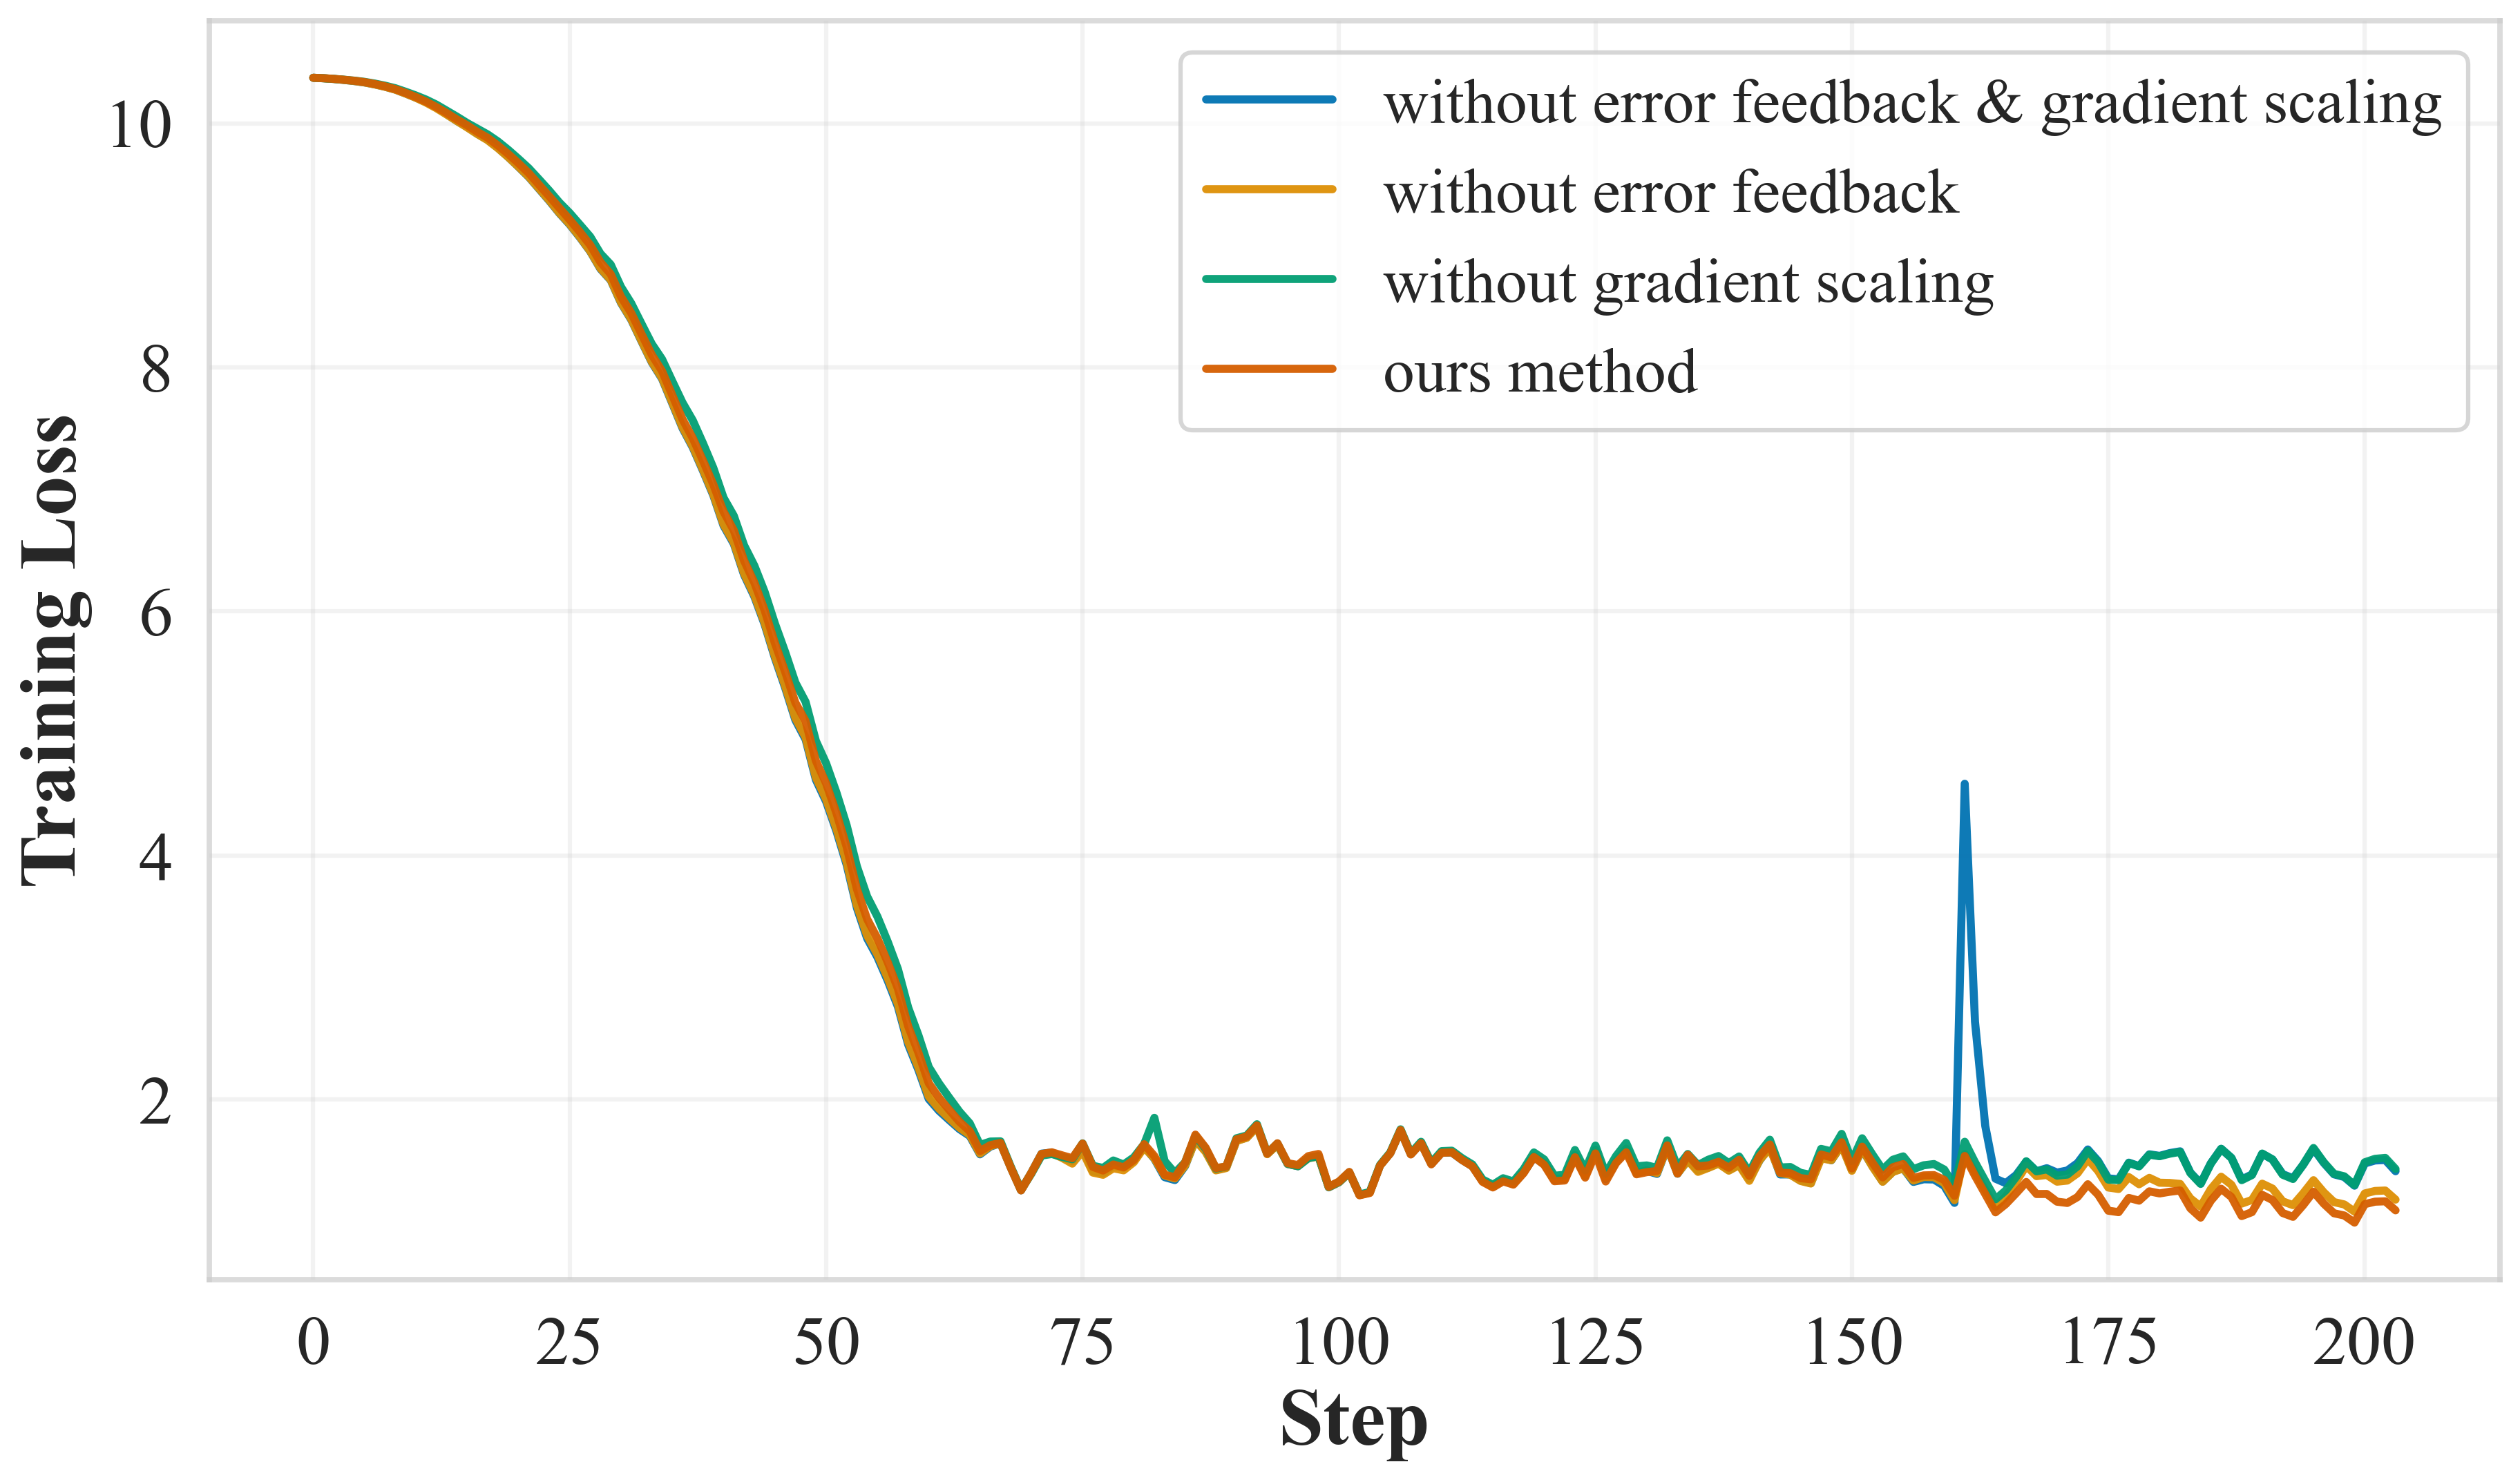
\includegraphics[width=\columnwidth]{images/json_curves_by_steps_ablation.png}
    \caption{Training loss changes with step under different ablation settings.}
    \label{fig:loss_ablation}
\end{figure}

% 我们针对本文的两个核心机制进行了消融实验，如\ref{fig:loss_ablation}所示，对于设置完全一致的训练，不使用gradient scaling方法，不使用error feedback策略，对于error feedback策略和gradient scaling策略都不使用这三个方法而言，相对于我们的原始方法在收敛程度、收敛稳定性上存在轻微的损失。对于不使用gradient scaling和error feedback方法而言，最终loss的收敛程度有所退化；而二者均不使用的情况下，在训练已经收敛的时候出现了明显的spike，预示着训练稳定性遭到了一定程度的挑战。

We conduct ablation experiments on the two core mechanisms of this paper. As shown in \ref{fig:loss_ablation}, for training with identical configurations, the three variants: without gradient scaling, without the error feedback strategy, and without both gradient scaling and error feedback exhibit a slight degradation in terms of convergence degree and convergence stability compared to our original method. Specifically, the variant without gradient scaling and error feedback shows a degraded convergence in the final loss. For the variant without both mechanisms, obvious spikes appear after training has converged, indicating that the stability of the training is compromised to some extent.

% \subsection{Analysis and Discussion}

% Overall, the two figures jointly indicate that POLAR-SGD preserves step-wise convergence behavior while substantially improving wall-clock convergence. Compared with relaxed-synchronization baselines, POLAR-SGD exhibits a more stable training trajectory and reaches the low-loss regime faster in time, making it a practical and effective solution for large-scale training under realistic WAN-constrained Cross-DC settings.

% \subsection{Main Results}

% \paragraph{Throughput Improvement.}

% On the LLaMA-2 7B pre-training task, POLAR-SGD demonstrates a significant performance advantage. Our method achieves a \textbf{1.87$\times$ end-to-end throughput improvement} compared to the Standard DP+PP baseline. This result strongly validates the effectiveness of eliminating the pipeline stall by overlapping communication and computation.

% Nsight system profiling reveals that the baseline spends 34\% of each training step idle while waiting for All-Reduce communication. In contrast, POLAR-SGD reduces this communication overhead to just 7\%, which is primarily incurred during the pipeline ramp-up and ramp-down phases where overlap is not fully possible. This corresponds to a \textbf{4.8× reduction in communication-induced idle time}.

% \textbf{Model Convergence Quality.}

% Performance gains should not come at the expense of model quality. Figure~\ref{fig:loss_comparison} shows the training loss and validation perplexity curves for POLAR-SGD and the baseline method. We observe that POLAR-SGD exhibits a slightly slower convergence in the initial training phase (first 400 steps), which is attributable to the gradient asynchrony introduced by pipelined communication. However, this difference is transient—after 400 steps, POLAR-SGD's convergence curve aligns perfectly with the Standard DP+PP baseline, ultimately achieving identical model quality.

% This result is significant: despite the slight initial convergence fluctuation, our predictive error-correction mechanism successfully guides the model back to the optimal convergence path, ensuring that final performance is not compromised. More importantly, given that POLAR-SGD provides a 1.87× throughput improvement throughout training, even with the slight initial convergence difference, its end-to-end training efficiency (measured by wall-clock time to reach a target loss) still far exceeds the baseline. In other words, while POLAR-SGD may require slightly more steps to reach a given loss value, the substantially reduced per-step time results in significantly lower total training time.

% \subsection{Convergence and Model Quality}

% \subsection{Ablation Study}

% To isolate and verify the necessity of the predictive error-correction (EC) mechanism, we conducted an ablation study. We compare the full POLAR-SGD method against the "Pipelined (w/o EC)" variant, which disables the correction mechanism.

% The results show that while the "Pipelined (w/o EC)" variant still achieves a performance benefit from pipelining, its model convergence is significantly impaired. On the WikiText-103 task, its final validation perplexity degraded from \textbf{10.38 (with POLAR-SGD) to 10.71}, a 3.2\% regression. This clearly demonstrates that without compensating for the gradient divergence introduced by asynchrony, the model deviates from the optimal convergence path, leading to a drop in final performance.

% This ablation study provides strong evidence that the predictive error-correction mechanism is an indispensable component of POLAR-SGD. It is the key that enables our aggressive communication overlap strategy to be practical, ensuring that the significant gains in throughput do not sacrifice the final model quality.